% public reference 
% https://indico.cern.ch/event/782953/contributions/3482451/attachments/1888308/3114226/20190801-DPF2019-ALW-final.pdf
% https://inspirehep.net/literature/1790595
% https://cms.cern/detector/detecting-muons/cathode-strip-chambers

% https://indico.cern.ch/event/663474/contributions/3060096/attachments/1681230/2701095/ICNFP2018_Overview_CMS_performance.pdf
% https://twiki.cern.ch/twiki/bin/view/CMSPublic/MuonDPGPublic160729
% https://twiki.cern.ch/twiki/bin/view/CMSPublic/MuonDPGResults

The CMS Cathode Strip Chambers (CSC) are a group of 540 gas ionization chambers located in the CMS endcaps. The CSC cavities are filled with a gas mixture composed of Ar, $CO_{2}$ and $CF_{4}$, and detect muons via ionization of this gas mixture. A diagram showing a CSC and its mechanism for muon detection is shown in Figure \ref{fig:CSC_Diagram}. 

\begin{figure}[H]
    \centering
    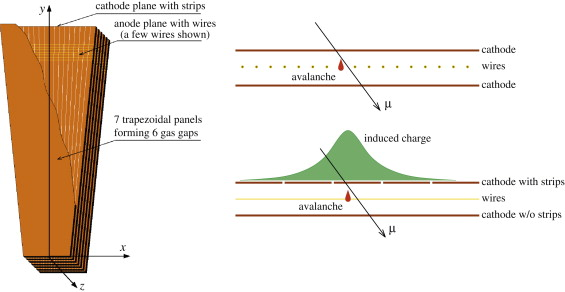
\includegraphics[width=0.7\textwidth]{Images/CMS/Muons/CSC/CSC_image.jpg}
    \caption{Muon detection in the CMS CSCs}
    \label{fig:CSC_Diagram}
\end{figure}

When an energetic muon from an LHC collision strikes a CSC, it knocks the electrons off of the atoms making up the CSC gas mixture. These electrons are forced to the anodes (positive ions forced to the cathodes) due to the presence of an electric potential, which produces an avalanche of electrons and thus a net charge.

The CSCs performed extremely well during Run 2, with an average segment reconstruction efficiency around 97\%, shown for the 2016 data taking year in Figure \ref{fig:CSC_2016SegHitEff}.

\begin{figure}[H]
    \centering
    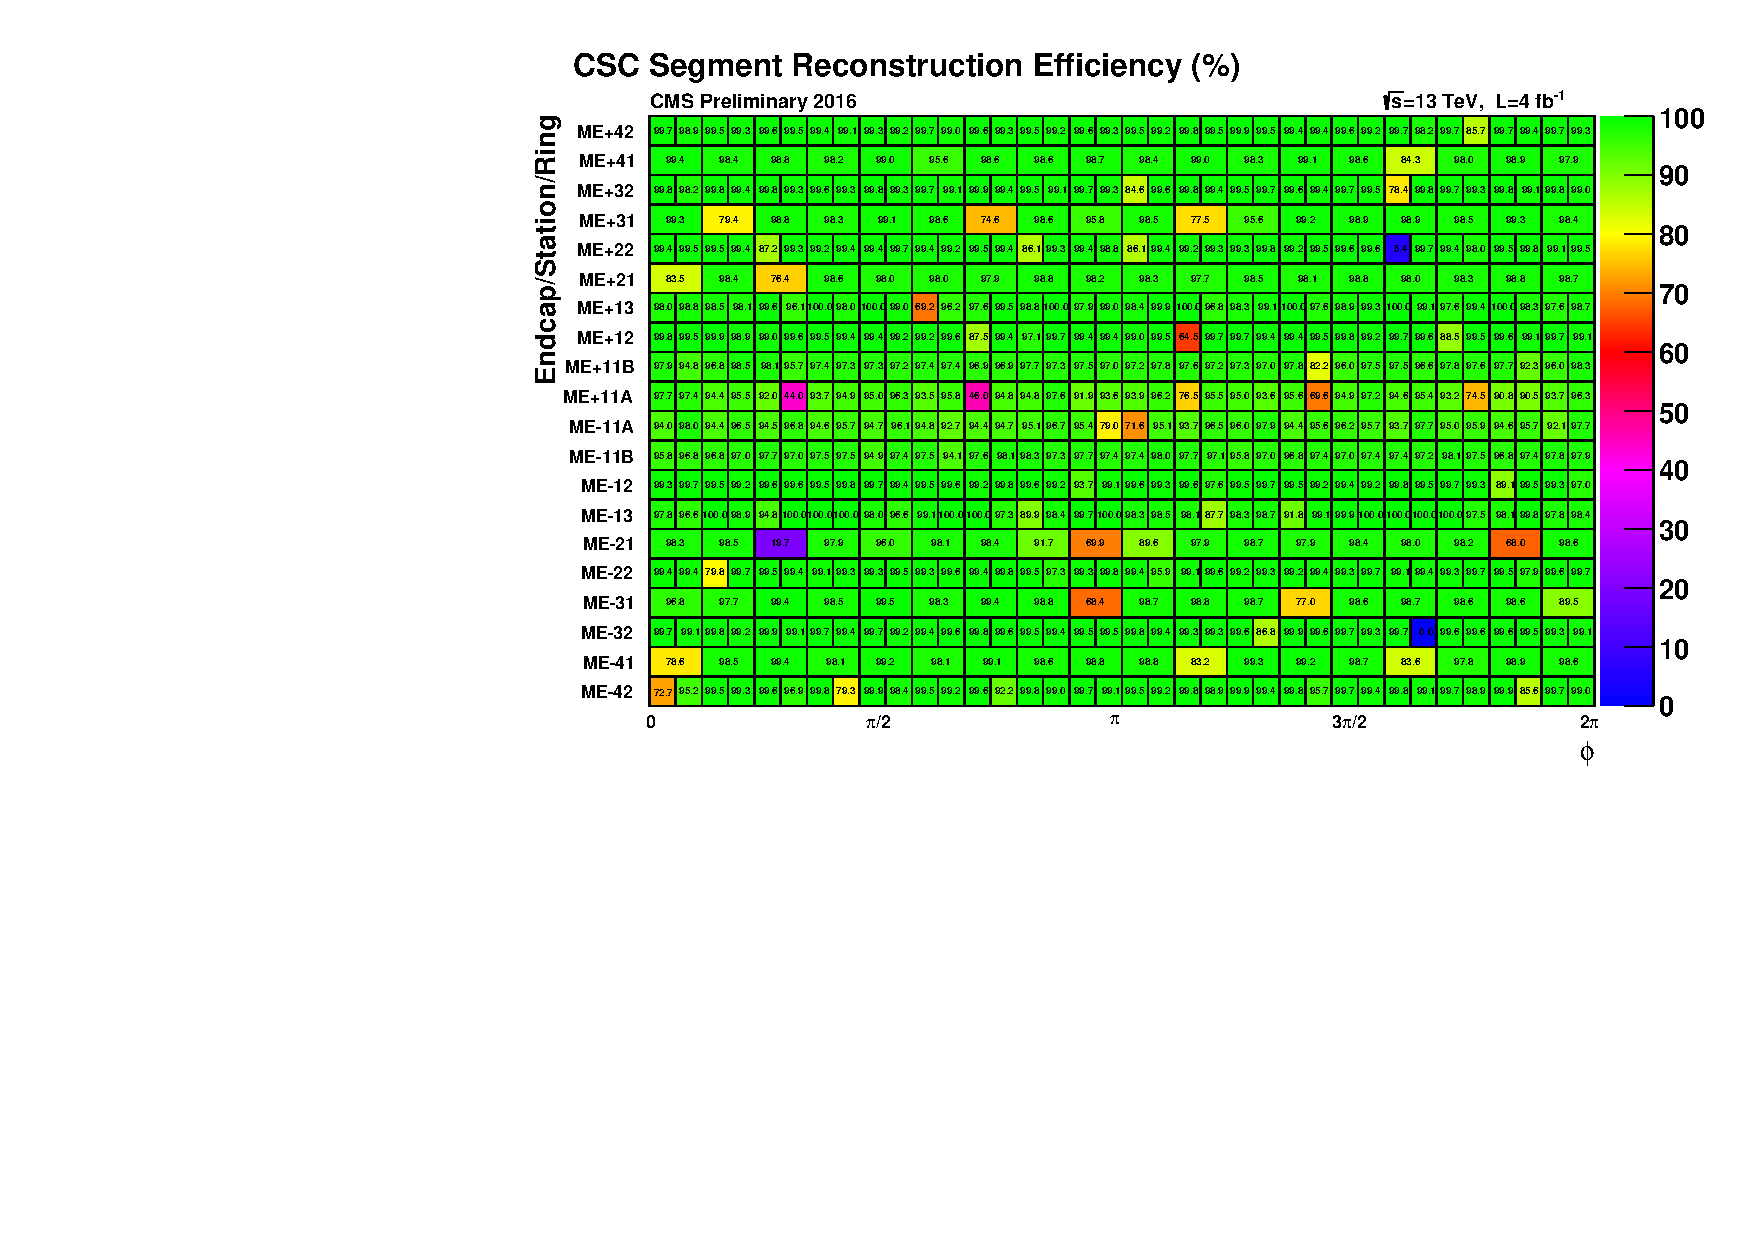
\includegraphics[width=0.85\textwidth]{Images/CMS/Muons/CSC/seg_eff_Muon_JSON_June22all_chambers_noErr.pdf}
    \caption{2016 CSC segment reconstruction efficiency.}
    \label{fig:CSC_2016SegHitEff}
\end{figure}